\documentclass[12pt]{article} 
\usepackage{amsmath} 
\usepackage[dvips]{graphicx}
\usepackage{multirow} 
\usepackage{geometry} 
\usepackage{pdflscape}
\usepackage{amsmath}
\usepackage[labelfont=bf]{caption} 
\usepackage{setspace}
\usepackage[running]{lineno} 
% \usepackage[numbers,sort]{natbib}
\usepackage[sort]{natbib} 
\usepackage{array}
\usepackage[table]{xcolor}
\usepackage{xr}
\usepackage{indentfirst}

\newcommand{\methods}{\textit{Materials \& Methods}}
\newcommand{\SI}{\textit{Appendix}~}

\topmargin -1.5cm % 0.0cm 
\oddsidemargin 0.0cm % 0.2cm 
\textwidth 6.5in
\textheight 9.0in % 21cm
\footskip 1.0cm % 1.0cm

\usepackage{authblk}


\title{Species motif participation provides unique information about species risk of extinction}

\author{Alyssa R. Cirtwill$^{1*\dagger}$, Anna \r{A}kesson$^{2*}$, Kate L. Wootton$^{3}$, Anna Ekl\"{o}f$^{2}$} 
\date{
\small$^1$Spatial Foodweb Ecology Group\\
Research Centre for Ecological Change\\
Organismal and Evolutionary Biology Research Programm\\
Faculty of Biological and Environmental Sciences\\
University of Helsinki, Helsinki, Finland\\
\medskip
\small$^2$Department of Theoretical Biology, Chemistry, and Physics\\ 
Link\"{o}ping University, Link\"{o}ping, Sweden\\
\medskip
\small$^3$ School of Biological Sciences\\
University of Canterbury, Christchurch, New Zealand\\
\medskip
* Joint first authors\\
\medskip
$^\dagger$ Corresponding author email: alyssa.cirtwill@gmail.com\\
}

% Limit is 8500 words.
% Currently c. 9000
\begin{document} 
\maketitle 
\raggedright

\setlength{\parindent}{15pt} 

\section*{Running headline}
Motif participation describes extinction risk

\clearpage

\section*{Summary}


    \indent{1. Bottom-up effects of disturbances to basal resources can strongly affect the persistence of consumers, but it is difficult to predict which species will be most affected by increasing disturbance.} \\
    2. A species' position in a food web (e.g., its trophic level or number of prey) is known to affect its ability to persist following disturbance.
    3. We therefore expect that a species' participation in three-species motifs --meso-scale structures which provide information on a species' direct and indirect interactions-- will also be related to its probability of persistence.\\
    4. We show that consumer species which participate more frequently in the direct competition motif and less frequently in the omnivory motif generally have higher probability of persistence following disturbance to basal resources.\\
    5. However, both the strength of the disturbance and the overall network structure (i.e., connectance) affect the strength and direction of relationships between motif participation and persistence.\\
    6. Motif participation therefore captures important trends in species persistence and provides a rich description of species' structural roles in their communities, but must be considered in the context of network structure as a whole and of the specific disturbance applied.


\section*{Key-words}
    food web, degree, trophic level, omnivory, competition

\clearpage
\begin{spacing}{2.0}
% \linenumbers

\section*{Introduction} %New

    The loss of a species in a food web can, due to the mutual dependencies among species,  trigger a cascade of additional (secondary) extinctions. 
    A species' risk of going secondarily extinct is known to depend on its position within a food web~\citep{Santos2021,curtsdotter2011robustness, dunne2009cascading, Eklof2006}.
    For example, species with high trophic levels (long paths to basal resources) and low in-degree (few prey) are generally more likely to go extinct~\citep{Allesina2012,binzer2011susceptibility, Eklof2006}.
    Species with low in-degree are more vulnerable to extinction because they have few alternative resources if a prey species is lost, while those with high trophic levels are vulnerable to the loss of any species along the path from basal resource(s) to the focal species.
    As well as these simple measures of food-web position, it has also been proposed that a species' participation in \emph{meso-scale structures} (which take into account the species' direct and indirect interactions) are related to its persistence~\citep{Cirtwill2022Oikos}.
    
    
    One way to describe a species' participation in such meso-scale structures is using its participation in the set of \emph{motifs} of a given size~\citep{Cirtwill2015a,Cirtwill2018FoodWebs}.
    Motifs --unique patterns of $n$ interacting species-- correspond to different sets of direct and indirect interactions and provide a holistic description of a species' place in a network~\citep{Stouffer2007,Stouffer2012}.
    Like degree and trophic level, a species' \emph{motif participation} (the vector of frequencies with which it appears in each motif) can easily be calculated once the structure of the network is known.
    However, unlike in-degree and trophic level, which focus only on direct prey of the focal species or on the lengths of paths between the focal species and basal resources, motif participation also incorporates information on the positions of focal species' interaction partners.
    Two species might both have two prey and a trophic level of 3, but they might have quite different motif participation if one species's prey are strict specialists and the others' prey are generalists.
    Importantly, since specialists are usually more vulnerable to extinction than generalists, the predator of specialists will be more likely to lose prey and go extinct itself than will a predator of generalists.
    Therefore, a species' motif participation profile captures the indirect interactions that affect the species, thereby capturing important structures that are missed by larger- or smaller-scale descriptions of the network.
    As such, motif participation may complement degree and trophic level to more fully predict species' extinction risk.
    
    
    Here, we focus on persistence after the loss of plants or other basal resources, i.e., the effects of bottom-up disturbances.
    The plant community is the foundation upon which the myriad species in food webs depend for their survival, and loss of basal resource diversity typically causes declines in both abundance and richness of all types of consumers~\citep{scherber2010bottom,Dobson2009food, Mduma1999food, Georgiadis2007}.
    Moreover, disturbances to the plant community have been shown to affect important ecosystem properties such as primary \citep{Hector1999} and secondary production \citep{borer2012plant}, soil respiration and carbon cycling \citep{chen2019plant}, and consumer diversity \citep{scherber2010bottom, Baiser2016,li2020bottom}.
    It is therefore critically important to understand how bottom-up effects of disturbance affect the rest of the food web.
    As well as identifying patterns of motif participation that are associated with greater or lesser ability to persist after a loss of basal resources, we are particularly interested in whether the strength of  disturbance affects relationships between motif participation and persistence.
    For example, participation in one motif might be associated with greater probability of extinction after a mild disturbance but be associated with less risk of extinction when when more basal resources are lost if the direct and indirect interactions within the motif amplify the effect of small disturbances but also provide the species with alternatives when disturbances are strong.

    

    %There are 13 possible three-species motifs (the most commonly-used size for food web analyses)~\citep{Milo2004,Stouffer2007,Stouffer2012,Cirtwill2015a}, 
    We define motif participation using three-species motifs, which are the most commonly-used size for food web analyses~\citep{Milo2004,Stouffer2007,Stouffer2012,Cirtwill2015a}. 
    Four of these motifs, namely the three-species chain, apparent competition, direct competition, and omnivory, are especially interesting as they are by far the most common in empirical networks~\citep{Stouffer2007, Borrelli2015a, giling2019plant}.
    These four motifs also have clear ecological interpretations.
    The three-species chain indicates vertical flows of energy and biomass in a network and captures the possibility of indirect interactions across multiple trophic levels (e.g., between a plant and a predator of the plant's herbivore).
    The direct competition motif, where two consumers share the same resource, captures the possibility of indirect interactions between consumers (e.g., by depletion of the shared resource). 
    The apparent competition motif, where a predator consumes two resources, can include indirect effects between prey (e.g., by boosting predator populations) in a top-down context, but only includes direct bottom-up interactions.
    Finally, the omnivory motif, where a predator consumes the same resource as its prey, includes captures the potential for a plant to have both direct and indirect effects on the predator. 
    
    
    %\subsection*{Here we test...}
    Here, we analyse whether a consumer's risk of secondary extinction after removal of basal resources depends on the consumer's motif participation and how this relationship varies with the severity of disturbance.
    To provide context for these results, we also consider how a consumer's risk of secondary extinction varies with the overall structure of the network, described by the frequency of motifs, network size, and network connectance.
    Finally, because measures of food-web position are not independent, we identify how species' motif participation varies with overall network structure and with in-degree and trophic level.


\section*{Methods}

    \subsection*{Network construction and describing species roles}

        We generated simulated networks using the niche model, which has been shown to recreate the structure of empirical networks well~\citep{Williams2000,Stouffer2007}.
        To capture a range of network architectures similar to those in well-studied empirical networks~\citep{Dunne2002,Dunne2002e}, we simulated networks with sizes (S) ranging from 50 to 100 species (in steps of 10) and connectances (C) ranging from 0.02 to 0.18 (in steps of 0.04). 
        All networks were generated using the function ``nichemodel'' within the Julia~\citep{Bezanson2017julia} package \emph{BioEnergeticFoodWebs}~\citep{bioenergfw,Delmas2017}.   
        For full details and a comparison to empirical networks, see \emph{Appendix S2}.
        We removed any biologically unlikely networks (i.e., those with extremely long paths between any consumer and basal resources~\citep{Borrelli2014}; \emph{Appendix S2}) and replaced them with new simulated networks, repeating the process until we obtained 100 suitable networks in each combination of size and connectance.

        
        % To make the simulated networks compatible with the Bayesian simulation framework, all networks were rendered acyclic following~\citet{Allesina2009functional} and species topologically sorted from lowest to highest trophic level (\emph{Appendix S2}). 
        %  These processing steps allow the strictly bottom-up calculation of probability of persistence.
        We then described each consumer species' motif participation role in each of these simulated networks before applying any disturbance. 
        A species' ``motif participation role'' (Fig.~\ref{fig:concept}) is the frequency with which the species appears in each of the motifs present in a network~\citep{Stouffer2012}.
        As only four unique three-species motifs can appear in acyclic networks, these are four-dimensional vectors. 
        Here we are interested in the relative frequencies of each motif rather than the total number of motifs and therefore normalized participation vectors by dividing each count by the total number of motifs the species appears in (such that the vector for each species sums to 1).
        Note, however, that this normalization does not necessarily control for differences due to degree or connectance~\citep{Cirtwill2022Oikos}. 


        We also calculated two simpler measures of a species' role within its community.
        In-degree is a species' number of prey.
        Trophic level (shortest trophic level; STL) is the length of the shortest food chain between the focal species and any basal resource~\citep{Williams2004}.
        Both simple role measures were calculated in R~\citep{R} using the same algorithm as~\citet{Eklof2013}.

        
        Finally, to provide context for species' motif participation, we calculated network ``motif profiles'': four-dimensional vectors of the number of each three-species motif in each network~\citep{Stouffer2012}.
        Together with network size and connectance, these motif profiles describe the structure of the whole network rather than how a particular species participates in the community.
        To separate differences in motif structure from differences in network size or connectance (larger and more-connected networks contain more motifs), we normalized motif profiles by dividing the count of each motif by the total count of all motifs. 
        We calculated species' motif participation using the Python package \emph{pymfinder}~\citep{pymfinder}.

    
    \subsection*{Modelling secondary extinction using Bayesian networks}


        Traditionally, there are two main approaches for studying secondary extinctions (i.e., extinctions of species that were not directly disturbed). 
        First, there are topological models, based only on food web structure \citep{dunne2009cascading}. 
        Here, extinctions only affect other species in the network once a consumer has lost all of its prey and therefore must go extinct. 
        The second approach uses dynamical models which explicitly simulate population dynamics using a system of differential equations \citep{binzer2011susceptibility}. 
        Dynamical models take changes in prey or predator densities into account when calculating the densities of other species in the network. 
        This additional detail means that realistic processes such as indirect interactions can be included, but also means that dynamical models are highly parameter intensive and simulations are much more time-consuming than topological models. 
        
        
        A middle‐ground approach for simulating secondary extinctions is to use Bayesian networks, which are much more computationally efficient and facilitate the analysis of larger networks than is practical for dynamical models \citep{Eklof2013,Haussler2020}. 
        In this framework, a consumer's probability of extinction depends on the fraction of resources lost ($f = k/n$ for a species with $n$ resources, of which $k$ have gone extinct) and on a baseline probability of extinction ($\pi$) which captures factors affecting the focal species' extinction probability that are not related to the network structure (e.g., disease or stochastic extinction of small populations).
        Importantly, the greater speed of the Bayesian network framework allows us to simulate a range of disturbance severities rather than single species removals as in many previous studies (e.g.,~\citealp[]{Memmott2004,Staniczenko2010,Dunne2004,Cirtwill2022Oikos}).
        Moreover, Bayesian network simulations are less parameter-intensive than dynamical models, meaning that they are less sensitive to assumptions made in the modelling process~\citep{Eklof2013}.

        % Mention acyclic resstriction here.
        One limitation to Bayesian networks is that consumers do not affect the extinction probabilities of their resources (i.e., only bottom-up effects are included).
        Nevertheless, Bayesian networks do capture the vast majority of secondary extinctions obtained from fully-fledged dynamical models including top-down and bottom-up effects~\citep{Eklof2013}, and as such are a good proxy for analysing species persistence following extinctions of primary producers in complex food webs.
        As our focus in this study is on bottom-up effects from disturbance of basal resources, Bayesian networks will capture the secondary extinctions we are interested in.

        
        Bayesian networks also require the creation of acyclic networks so that a strict bottom-up sequence can be followed. 
        This means that cycles where species A eats species B and vice versa or where A eats B eats C eats A must be broken (see \emph{Appendix SX} for details).
        Since cyclic and acyclic versions of a network have the same properties in terms of secondary extinctions and the effects on network robustness are very limited~\citep{Allesina2009functional}, this change will not strongly affect consumers' extinction risk in our simulations.

        
        The removal of cycles also affects which motifs can appear in the network. 
        Any motif which contains a cycle is impossible in an acyclic network.
        This means that only four motifs can appear: apparent competition, direct competition, omnivory, and the three-species chain.
        Fortunately, they are also the motifs that are most common in empirical networks (\citealp[]{Stouffer2007}, have been most studied in isolation (e.g.,~\citep{Hastings1991,Holt1987,Bascompte2005,Polis1989,Zabalo2012,Lefevre2009,Holt1997,Kondoh2008,McKinnon2013,Laws2013}), have the clearest ecological interpretations and, because of these three properties, are of greatest interest to us.


        \subsubsection*{Modelling consumers' risk of secondary extinction}
        
        The response of the consumer to changes in $f$ can take any form (\emph{Appendix S1}). Here we use a sigmoid non-linear function ($\alpha > 1, \beta > 1$), the type of response that most accurately captures the secondary extinctions produced by dynamical models (\citealp[]{Eklof2013}).
		The probability of extinction for each species $i$ can therefore be represented using the cumulative density function of a beta distribution:
		\begin{equation}
		P(\lnot i|f) = \pi + (1 - \pi) \frac{B(f;\alpha,\beta)}{B(\alpha,\beta)}.
				\label{betafunc}
        \end{equation}
		
		If all resource species of a consumer \textit{C} are present ($f = 0$), the extinction probability will be $P(\lnot C|f) = \pi$. 
		Similarly, if all resources are extinct ($f = 1$), the extinction probability $P(\lnot C|f)$ will be equal to 1 and the consumer will go extinct.
		If the fraction $f$ is neither 1 nor 0, the non-linear sigmoid curve will determine the response of the consumer, which will be more severe if the fraction of resources lost is high. This will in turn affect the extinction probability $P(\lnot C|f)$.
		For basal resources, we assume that the abiotic resources they require are always available and therefore $f=0$. 
		Following Equation \ref{betafunc}, the extinction probability of a basal resource will only depend on $\pi$.
		Note that we here assume that only the fraction, and not the identity, of the resources lost is important. 
		However, the model can easily be modified to incorporate weighted resource interactions \citep[see][]{Eklof2013}.
		
		
		% how we calculate persistences 
        Beginning with basal resources and working systematically up through the food web, we use Equation \ref{betafunc} to calculate each species $i$'s probability of extinction $P(\lnot i|f)$.
        Using this probability, we then perform Bernoulli trials to determine whether the species goes extinct or not. 
        Species are considered extinct if a random number drawn from a uniform distribution $[0-1]$ is less than $P(\lnot i|f)$.
        These simulated extinctions are used when calculating the fraction of resources lost $f$ for each consumer.
        This allows us to update Equation~\ref{betafunc} with information on extinctions of a focal consumer's resources and simulate bottom-up effects. As this method is probabilistic, we repeat these calculations 100 000 times per network, with unique random draws.
        For each species, we then define probability of persistence (hereafter `persistence') as the fraction of simulations in which the species persists. 
        While there are methods for solving Bayesian networks exactly \citep{Eklof2013}, for larger networks the numerical evaluation above is highly efficient and produces close to identical results \citep{Haussler2020}.
		
	
		
        \subsubsection*{Disturbance scenarios}
        
            In our un-disturbed scenario, all species had an extinction probability of $\pi = 0.1$. 
            To simulate various threats to basal resources, making some species more vulnerable to extinction, we increase all basal species' probability of extinction from $0.10$ to $0.5$, in steps of $0.08$. 
            The highest disturbance level, $\pi = 0.5$, corresponds to basal species having a 50\% risk of going extinct. 
            Consumer species retained $\pi=0.1$ in all cases.


	\subsection*{Statistical analysis} 
	% Appendix 3, with numbered subheadings.

        We first tested 1) how consumer species persistence varied with motif participation and the severity of disturbance.
        For context, we also test 2) how a consumer's persistence varies with other measures of network structure and a species' place within it.
        As different measures of network structure are not independent since all describe the same network, we also 3) relate species' motif participation to large-scale network structure and to species in-degree and trophic level.
        All analyses are briefly described below and were performed using  R~\citep{R} package. % \emph{lmerTest}~\citep{lmerTest}.
        % , \emph{MuMIn}~\citep{MuMIn}, and \emph{vegan}~\citep{vegan}.
        See Appendix \emph{S3} for details. 

        
        \subsubsection*{1) Consumer persistence and motif participation}

            To test whether a consumer's risk of extinction was associated with the frequency of each motif in its participation vector (hereafter simply `participation in motif X') and whether this relationship varied with the strength of disturbance, we fit four general linear models with binomial error distribution (GLMs; one per motif included in the Bayesian networks):
            \begin{equation}
            \Psi_{ink} \approx \rho_{i} + \pi_{k} + \rho_{i}\pi_{k} ,
            % S_{n}C_{n} + N_n,
            \label{propreq}
            \end{equation}
            \noindent where $\Psi_{ink}$ is the persistence of species $i$, belonging to network $n$, during disturbance level $k$, $\rho_{i}$ is the proportion of the role of species $i$ that is made up by the focal motif, and $\pi_k$ is the probability of extinction for a basal resource in disturbance level $k$.
            All predictors were centered and scaled before fitting the models.         

            
            
            Initially, we fit general linear mixed-effect models (GLMMs) also including random  intercepts for the species richness and connectance of network $n$ and for network identity.
            As these models were singular, we removed each random intercept in turn and re-fit the model until it converged.
            In all four cases, the convergent model did not retain any random effects.
            We attempted to fit a PERMANOVA test relating a species' motif participation vector as a whole to its persistence, but the assumption of equal variance among groups was violated and we therefore do not report the results of this test.
            
            
            To test whether these general trends were consistent across networks, we visually examined the distribution of slopes of simplified regressions fit to a single network and level of disturbance.
            These models included only participation in the focal motif ($\rho_{i}$ above) and again used a binomial error distrubution.
            To aid in interpretation of these single-network models with respect to network size and connectance, we fit an additional set of GLMs including proportion of motif, strength of disturbance, network size, and connectance across all networks (\emph{Appendix S6}).



        \subsubsection*{2) Consumer persistence and other network structure metrics}

            The overall structure of a network could also affect consumers' ability to persist following a disturbance.
            Here, we describe the overall network structure using the frequency of each motif in the whole network (i.e., the network's motif profile) as well as network size and connectance (which were determined prior to network simulation).
            To test whether the frequency of particular motifs in the network profile were related to the average persistence of all consumers, we fit a set of four GLMs with binomial error distribution (one per motif):
                \begin{equation}
                    \overline{\Psi_{nk}} \approx \Bar{\rho}_{n} + \pi_{k} + \Bar{\rho}_{n}\pi_{k},
                    \label{netpropeq}
                \end{equation}
            \noindent where $\overline{\Psi_{nk}}$ is the mean persistence of all consumers in network $n$ at disturbance level $k$, $\Bar{\rho}_{n}$ is the proportion of the focal motif in the network's motif profile, and $\pi_k$ is the level of disturbance (probability of extinction for basal resources) as in equation~\ref{propreq}.
            As with the GLMs relating each consumer's persistence to its motif participation, we initially attempted to fit GLMMs including random effects of network size and connectance and network identity but removed these random effects in order to obtain non-singular models.


            We also confirmed previously-known relationships between persistence and other measures of network structure or a species' participation in the network.
            To identify the relationship between large-scale network structure and mean persistence within a network, and how the strength of disturbance might affect this relationship, we fit a GLM relating mean persistence to network size, connectance, disturbance, and their interactions.
            As the three-way interaction was significant, we did not simplify the model. 
            To confirm known relationships between persistence and in-degree or trophic level in our simulated networks and identify how they might vary with different strengths of disturbance, we fit two GLMs with binomial error distribution relating a consumer's persistence to in-degree or STL, disturbance, and the interaction between them (\emph{Appendix S3}, Eq. S2-3).
            As with the GLMs relating persistence to motif participation and motif profiles, we initially fit GLMMs including random effects of network size and connectance and network identity but removed these terms due to model singularity.



        \subsubsection*{3) Motif participation and other network structure metrics}

            Since a network's motif profile and a species' motif participation reflect the same network as other measures (size, connectance, degree, and trophic level), these measures are not independent. 
            We identified how the frequencies of motifs in the network's motif profile were related to network size, connectance, and their interaction using a set of four GLMs with binomial error distribution (Appendix \emph{S3}, eq. S4).
            We identified how the frequencies of motifs in a consumer's motif participation vector were related to network size, connectance, and their interaction using a similar set of four GLMs with binomial error distribution.
            Finally, we fit two additional sets of GLMs (eight total) relating participation in each motif to the consumer's in-degree or trophic level (Appendix \emph{S3}, Eq. S5-6).
        
        
\section*{Results}

    \subsection*{Species persistence and motif participation} 

        A species' probability of persistence (hereafter `persistence') was significantly related to its motif participation (Table S1, \emph{Appendix S4}).
        Across all levels of disturbance, species were more likely to persist if they participated more frequently in the direct competition motif and less frequently in the omnivory motif (Fig.~\ref{fig:prop_lmer_all}).
        The relationships between persistence and participation in the other two motifs varied with the strength of disturbance.
        At low levels of disturbance, species were more likely to persist if they participated more frequently in the three-species chain motif and less frequently in the apparent competition motif.
        These trends were reversed at high levels of disturbance.
    

        Within these overall trends, there was substantial variation in the relationships between persistence and motif participation between networks with different overall network structures (Fig.~\ref{fig:density_prop}).
        Networks with high and low connectances had different distributions of persistence-motif participation relationships, while network size had a much smaller effect (\emph{Appendix SX}).
        The relationship between participation in the omnivory motif and persistence was especially variable.
        Higher proportions of omnivory were associated with lower probabilities of persistence when connectance was low, regardless of network size or strength of disturbance.
        At moderate connectance, however, higher proportions of omnivory were associated with greater probabilities of persistence when disturbance was weak.
        In the most-connected networks, higher proportions of omnivory were associated with greater probabilities of persistence at all levels of disturbance.

        The relationships between persistence and participation in the other motifs were more consistent over different levels of connectance and network size.
        The persistence-motif participation relationships were strongest in networks with low connectance (Fig.~\ref{fig:density_prop}).
        For the apparent competition and three-species chain motifs, the direction of these relationships depended much more strongly on the strength of disturbance than on connectance.
        For the direct competition motif, persistence increased with increasing participation in the motif across all disturbance levels in networks with low and medium connectance.
        In networks with high connectance, however, the distribution of slopes for this relationship was centered around zero at all levels of disturbance.


    \subsection*{Persistence and other network properties}

        To understand the relationships between motif participation and consumers' probabilities of persistence, it is helpful to understand how persistence varies with other aspects of both consumer properties and network structure.
        
        Consumers with higher trophic level (STL) were less likely to persist (Fig.~\ref{fig:lm_CS}, Table S3, \emph{Appendix S6}).
        The relationship between in-degree and persistence depended on the strength of disturbance: higher in-degree was associated with greater persistence when basal species had low probability of extinction but lower persistence when basal species were highly likely to go extinct.


        The average persistence of all consumers was lower in networks with higher connectance, did not vary significantly with network size (Table S6, \emph{Appendix S10}), and  varied with the frequencies of different motifs in this profile.
        Specifically, average consumer persistence was higher in networks with higher proportions of the apparent competition motif, lower in networks with higher proportions of the omnivory motif, and was not significantly related to the frequencies of the three-species chain or direct competition motifs (Fig.~\ref{fig:lm_CS}, Table S4, \emph{Appendix S8}). 
        There was no significant interaction between the proportion of any motif in the network profile and level of disturbance (Table S4), \emph{Appendix S8}).


    \subsection*{Motif participation and other network properties}


        A species' motif participation varied with its position in the network and with overall network structure (Fig.~\ref{fig:motifs_vs_TL_and_deg}).
        Species with higher in-degree tended to have higher frequencies of participation in the omnivory motif and lower proportions of the other three motifs.
        Species with higher trophic levels tended to have higher proportions of apparent competition and three-species chains and lower proportions of omnivory and direct competition. 
        
        
        Omnivory motif participation generally increased with increasing connectance and network size, but decreased with increasing network size in the most-connected networks (Fig. S2 and Table S2, \emph{Appendix S5}).
        Participation in the apparent competition and three-species chain motifs decreased strongly with increasing connectance but showed little change with changing network size.
        Direct competition motif participation decreased with increasing connectance in small networks and increased with increasing network size in highly-connected networks, but showed little change with connectance in large networks or with network size in less-connected networks.

        
        The network's motif profile also varied with network connectance.
        Specifically, the proportion of the profile made up by the omnivory motif increased significantly  with increasing connectance while the proportions of the other three motifs decreased (though not significantly).
        No proportions of motifs in the profile were significantly related to network size.


\section*{Discussion}

    Identifying the species that are most and least likely to persist after a disturbance is a high priority for conservation efforts~\citep{Bottrilletal2008}. 
    Network structural properties such as connectance and measures of a species' position in the network such as degree and trophic level are known to affect species' vulnerability~\citep{Dunne2002, Eklof2006, PascualDunne2006,prill2005dynamic, bascompte2005simple,curtsdotter2011robustness, dunne2009cascading}, but are relatively coarse metrics.
    Defining a species' network role based on its participation in meso-scale motifs provides more nuanced information and may also predict extinction risk~\citep{Stouffer2007,Stouffer2010b,Simmons2019,Cirtwill2018FoodWebs}, but this potential is only beginning to be explored~\citep{Cirtwill2022Oikos}.

    
    Here we partially fill this knowledge gap by testing how the persistence of a consumer in a food web depends on its participation in four different motifs, and how this relationship varies with different levels of disturbance to basal resources.  
    We found that motif participation was related to a consumer's persistence in ways not fully explained by simpler measures of network structure. 
    Species participating more frequently in the direct competition motif and less frequently in the omnivory motif are more likely to persist, while the effects of participating in the apparent competition or three-species chain motifs depend on the strength of disturbance.


    Disturbance strength is often neglected when predicting risk of extinction, but proved important in our results.
    Several of the relationships we demonstrated between probability of persistence and species roles changed direction when moving from weak to strong disturbance.
    These simulation results echo other warnings about `tipping points' where previously beneficial traits can become risky~\citep{Latty2019,Golubski2016,Tylianakis2014}.
    For example, at low levels of disturbance a high degree may be protective since species can compensate if one or a few prey are lost. 
    At high disturbance, however, a high-degree species is likely to be affected by disturbances through many paths and therefore have lower persistence.
    This context-dependence contrasts with the general assumption that species with more resources will be less vulnerable~\citep{Allesina2012,binzer2011susceptibility}.
    These disturbance effects mean that efforts to define a set of target species for conservation interactions must take the current (and future) level of disturbance the community experiences into account.
    

    % Apparent competition as a case study that motifs are useful
    The relationship between persistence and participation in the apparent competition motif provides a good example of how motifs provide complementary information to simpler measures of a species' network role.
    Species with higher trophic levels tend to participate more frequently in the apparent competition motif and
    species with higher trophic levels generally have lower persistence~\citep{Eklof2006,Eklof2013}. We would therefore expect high participation in the apparent competition motif to also be associated with lower persistence.
    However, this is only true for low disturbance. 
    For high disturbance, we see the opposite relationship.
    This change in the persistence-apparent competition relationship across disturbance levels may be driven by the negative relationship between apparent competition and in-degree, and in-degree's negative relationship with persistence.
    However, it is not obvious when trophic level should be the most important predictor of persistence and when in-degree should be most important.
    Such simpler measures of species' positions in a network could therefore lead us astray either because they provide conflicting predictions or because our expectations are only reasonable for specific types or levels of disturbance.


    Omnivory motif participation likewise provides information about persistence that is not easily obtained from in-degree and trophic level.
    Although omnivory participation decreased with trophic level (as does persistence) and increased with in-degree (as does persistence, except at high disturbance), we found that greater omnivory participation was usually associated with \emph{lower} persistence-- contrary to what we would expect based on trophic level and in-degree.
    The exception to this pattern is found at high connectance, where increased omnivory participation was more likely to have a positive or neutral relationship with consumer persistence, especially at low disturbance levels (Fig. 3).
    This is consistent with other studies which have found the effect of omnivory to be highly context-dependent~\citep{bascompte2005simple, Monteiro2016} and particularly beneficial when interaction strengths are weak~\citep{Emmerson2004}.
    Although omnivory motifs tend to be less stable in isolation the the other motifs we consider here~\citep{Borrelli2015a}, when embedded in a network interactions with other species can stabilise even intrinsically unstable omnivory~\citep{Kratina2012}.
    Though we do not explicitly model interaction strengths, we do note that the greater number of interactions per species in high-connectance networks should lead to weaker interactions in general, as well as allowing many opportunities for additional interactions that could stabilise omnivory.
    

    
    

    % Caveats - expand on top-down effects a bit to make R2 happy
    There are limitations to the approach presented here.
    Most importantly, the Bayesian network framework operates on a strict bottom-up principle and therefore cannot include top-down effects in the extinction risk calculations~\citep{Eklof2013}. 
    Here our focus was to analyze bottom-up affects following disturbances to the basal resources, in which case the Bayesian network approach captures a majority of the secondary extinctions obtained in a fully-fledged dynamical model with much greater efficiency~\citep{Eklof2013}.
    If top-down effects are important for a particular empirical system, however, our simulations may not be accurate. 
    For example, although a recent study using a dynamical model to relate motif participation to persistence after a disturbance found similar trends for omnivory, participation in the direct competition motif was not universally positive~\citep{Cirtwill2021_inprep}.
    In particular, species which frequently appeared in the prey position of the direct competition motif tended to have shorter persistence times after disturbance in that study - possibly due to top-down effects from the pair of predators involved.
    However, as these two studies applied different types of disturbances, further study would be required to disentangle the effects of top-down and bottom-up effects on species with different motif participation, and how each relates to the type and strength of disturbance.
    Another potentially useful addition to future work would be to include species traits such as body size, which are related to both motif participation~\citep{cirtwill2018feeding} and extinction risk~\citep{Brose2017, curtsdotter2011robustness, Cardillo2005, Purvis2000} in empirical webs.

    
    
    \subsection*{Conclusions}
    
    Many ecologists, including ourselves, have argued that simple measures of species' roles within food webs are important for understanding species' extinction risk~\citep{Santos2021,curtsdotter2011robustness, dunne2009cascading, Eklof2006,binzer2011susceptibility}. 
    However, here we show that relationships between extinction risk and measures of a species' place in its food web are likely more complex, varying with the strength of disturbance and the overall network structure.
    This context-dependence means that even limited changes in network structure or the type of disturbance could change which species are most sensitive to disturbance. 
    As such, caution and increased attention to both network structure and the specifics of disturbance are needed for targetted conservation actions to be most effective. 
    
\section*{Acknowledgements}

    The authors thank Gy\"{o}rgy Barab\'{a}s for excellent discussion of the ideas in this manuscript. A{\AA} is supported by the Swedish Research Council for Sustainable Development Formas (\#2015-01262) granted to AE. ARC is supported by a Finnish Academy postdoctoral research grant (\#332999).

\clearpage    

\section*{Figures}
    

        \begin{figure}[hb!]
        \centering
        % 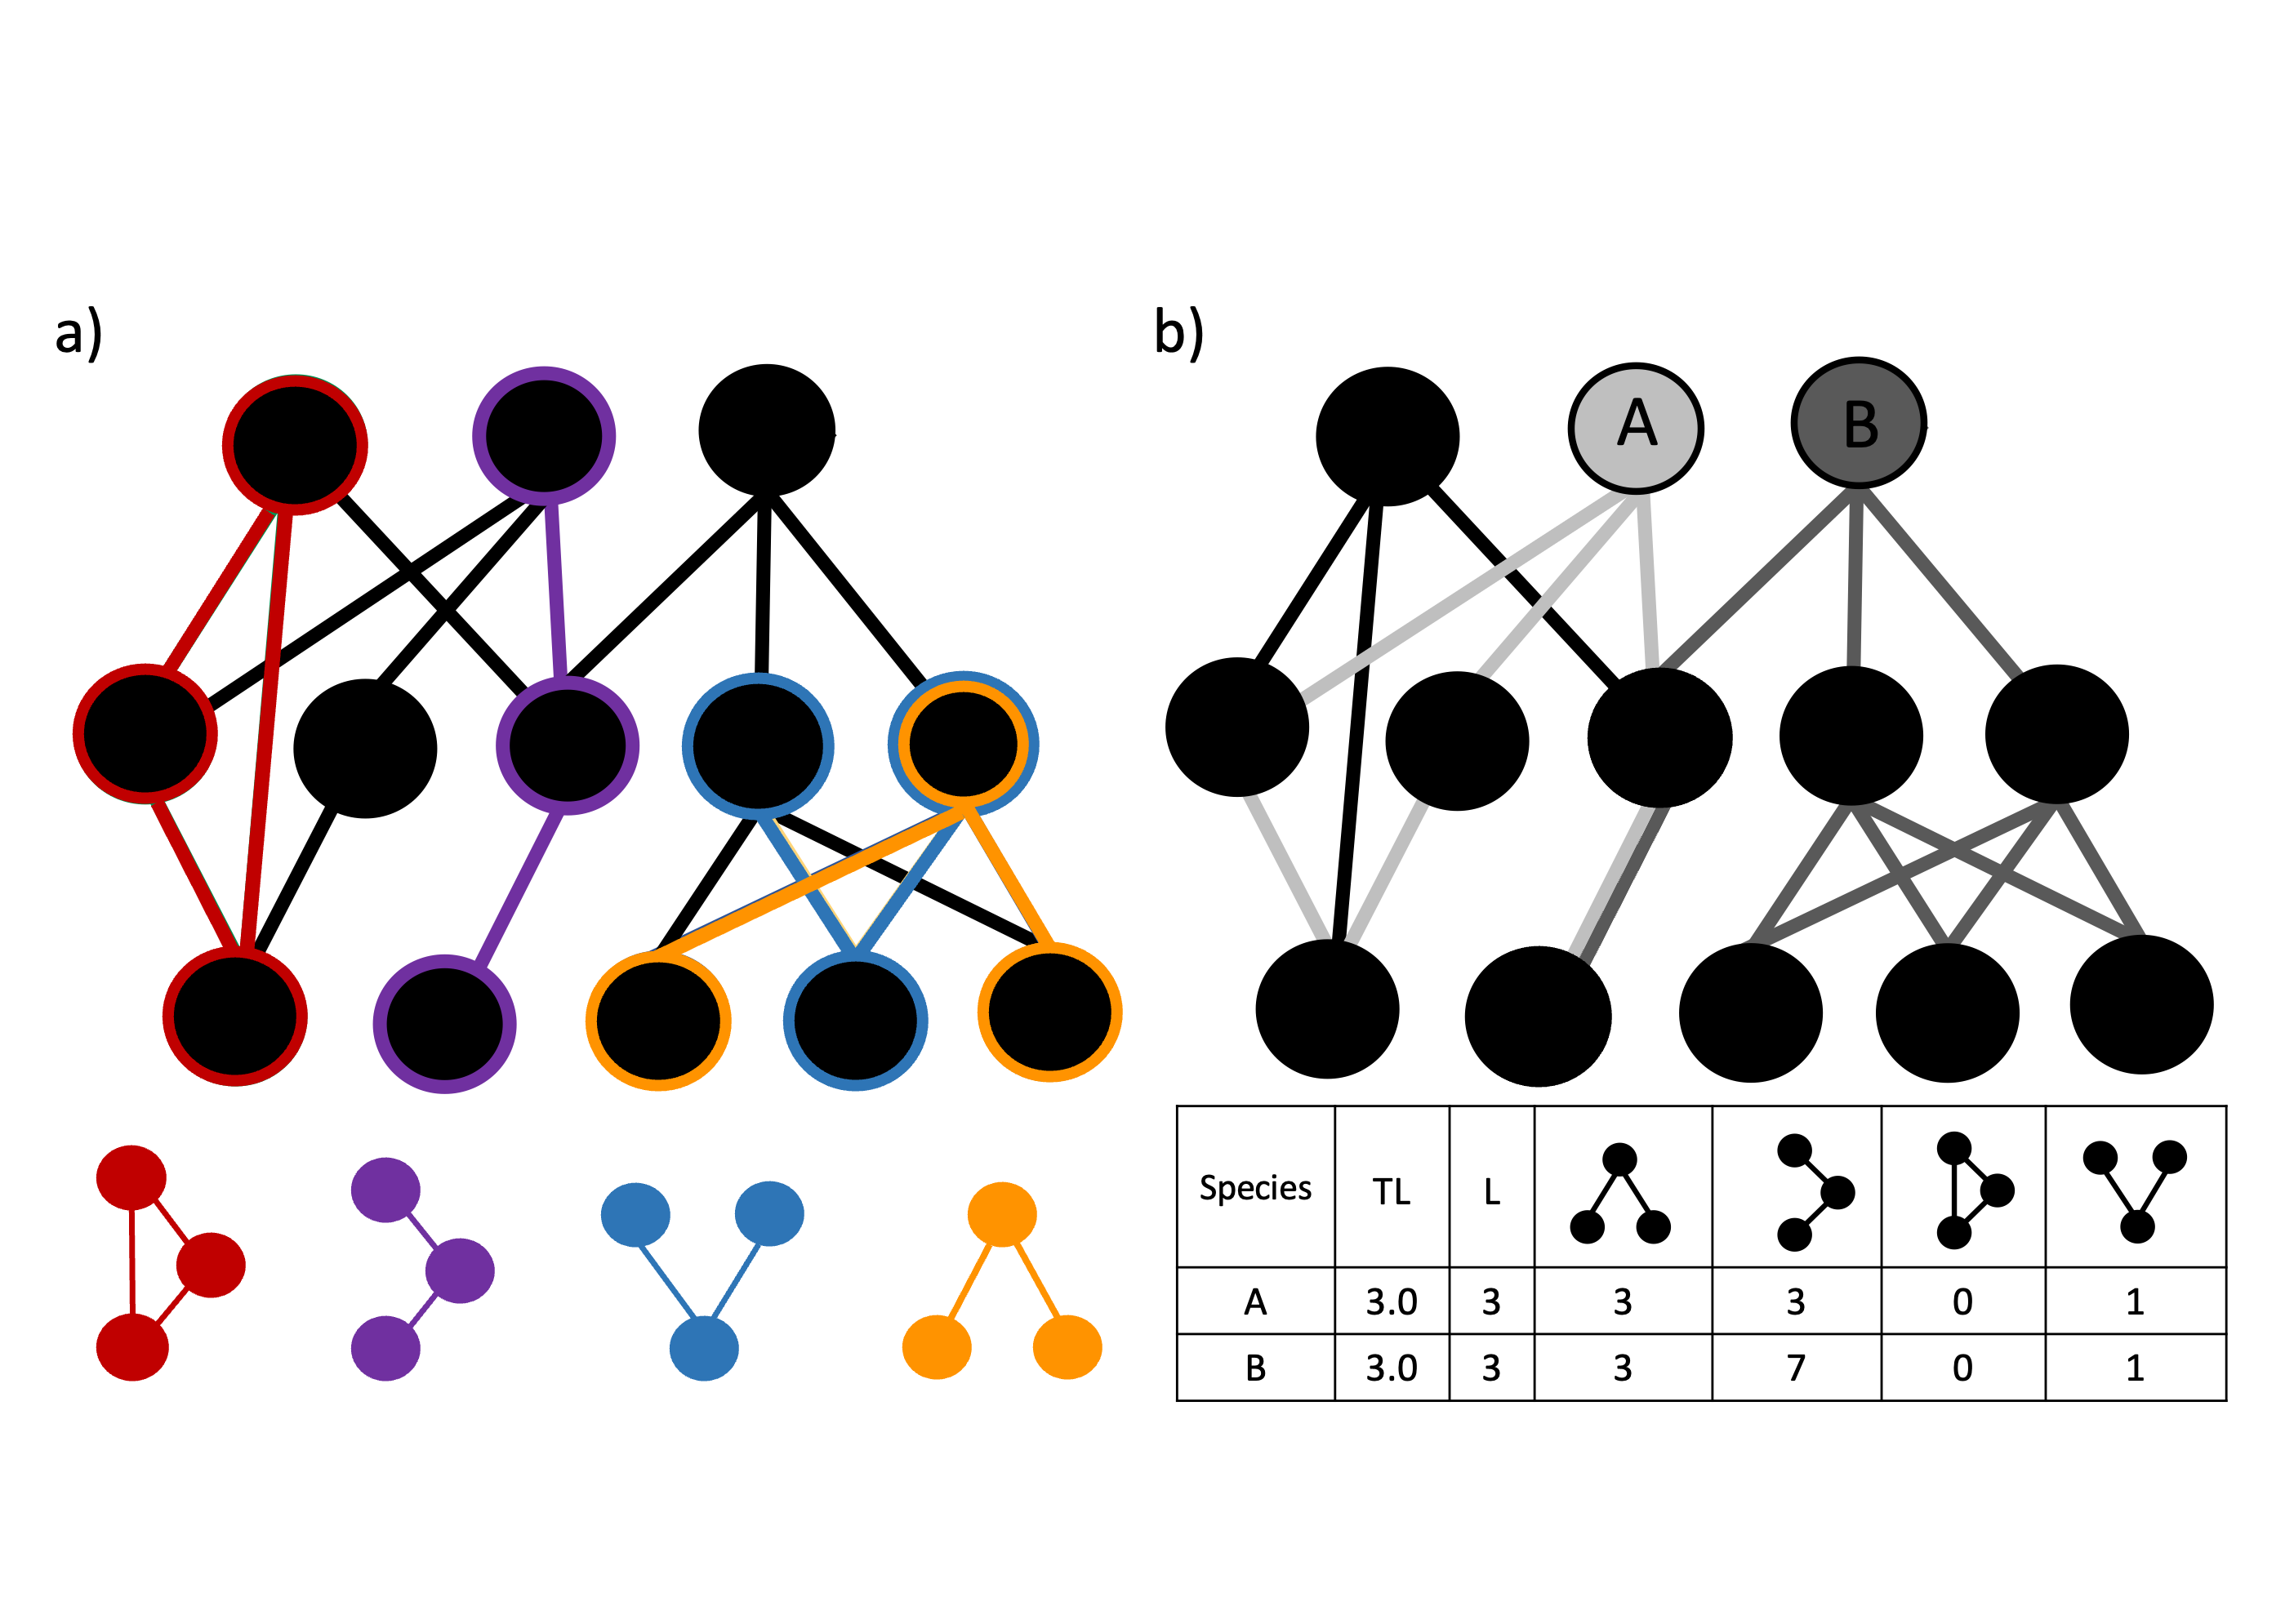
\includegraphics[width=.9\textwidth]{figures/Figure_1.png}
        \caption{Conceptual figure of a toy food web. \textbf{a)} This food web contains examples of the four motifs: apparent competition (blue), three-species chain (purple), omnivory (green), and direct competition (yellow). These motifs capture different ways in which disturbances to basal resources can propagate through the network. For example, a disturbance to the bottom species in a three-species chain will have a direct effect on the middle species but only indirectly affect the top species while a disturbance to the bottom species in an omnivory motif will have a direct effect on the middle species and direct and indirect effects on the top species. 
        Note that the nodes participate in more motifs than the ones highlighted and that a species' motif participation vector is the count of all motifs of each type in which the species appears. \textbf{b)} In the same food web, species with identical degree and trophic level can have different motif participation; here species A (light grey node with links in the same motif colored light grey) participates in only two chains while species B (dark grey node with its direct consumption links colored dark grey) participates in chains more than three times more frequently (see inserted table for counts of participation in all four motifs, giving the motif participation vector in parentheses). 
        Despite having equal degree and trophic level, species A may be at greater risk of going extinct than species B because of its dependence on specialist prey species. Two-thirds of the prey of species B are generalists and therefore more likely to survive a disturbance to basal resources. By including information about indirect interactions, motif profiles reflect this difference between species A and B while trophic level and degree do not.}
    \label{fig:concept}
    \end{figure}


    %     \begin{figure}[hb!]
    %     \centering
    %     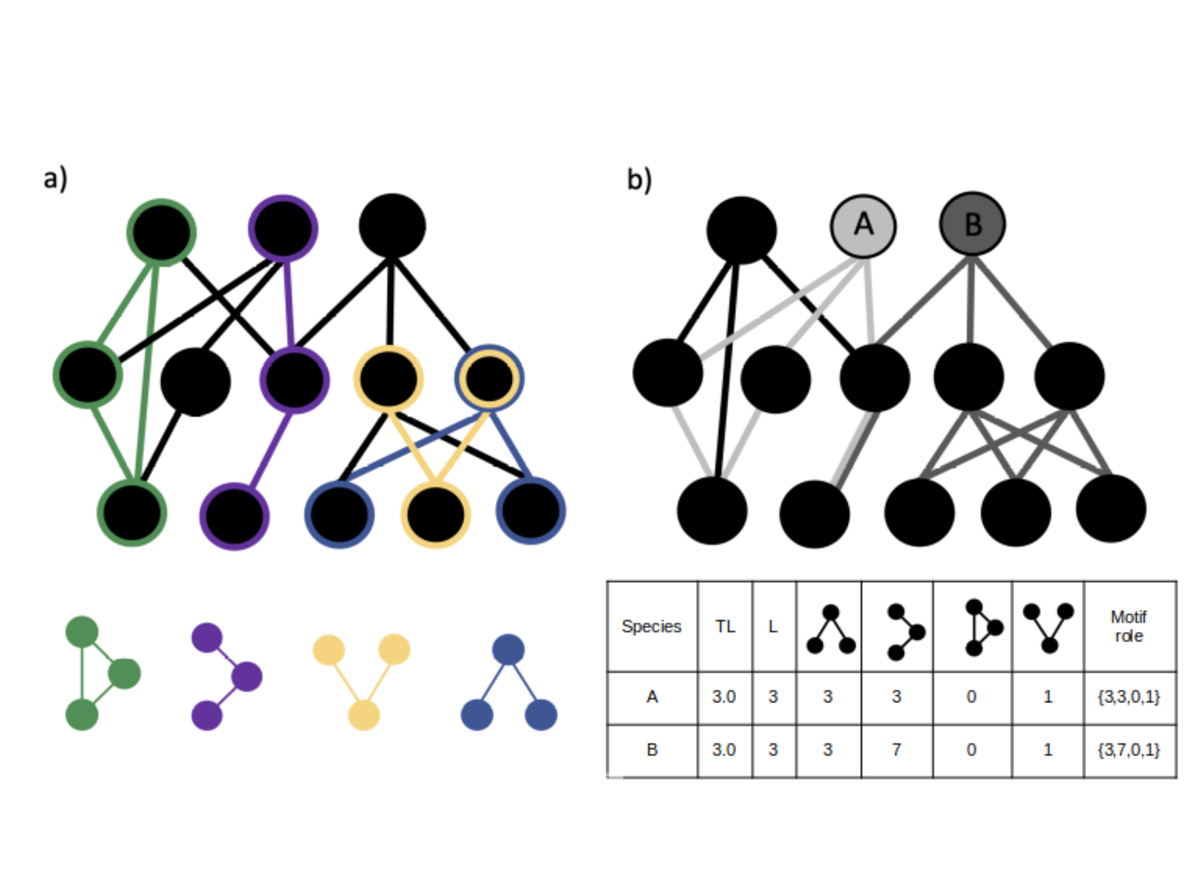
\includegraphics[width=.9\textwidth]{figures/concept_fig_ver2_edit.eps}
    %     \caption{Note motif participation vectors in the right-hand column of the box. I still think it's nice to show - can you add back into current Fig. 1?}
    % \label{fig:concept_wrongcolour}
    % \end{figure}

    
        \begin{figure}[hb!]
        \centering
        % \includegraphics[width=0.85\textwidth]{figures/persistence_motif_participation.eps}
        \caption{The effect of proportion of the role (x-axis) made up by various motifs (columns) on persistence (y-axis). The effect of participating in each motif is based on the fixed effects in Equation~\ref{propreq}. The different colored lines indicate the probability of extinction of basal species, from $\pi_{disturbed} = 0.1$ (top, purple; no disturbance) to $\pi_{disturbed} = 0.5$ (bottom, yellow; high disturbance). 95\% confidence intervals for each line are shown in grey. Note that omnivory made up a smaller proportion of species' roles than other motifs; lines are plotted over the observed ranges of motif participation.}
    \label{fig:prop_lmer_all}
    \end{figure}
        
    \begin{figure}[hb!]
    \centering
        % 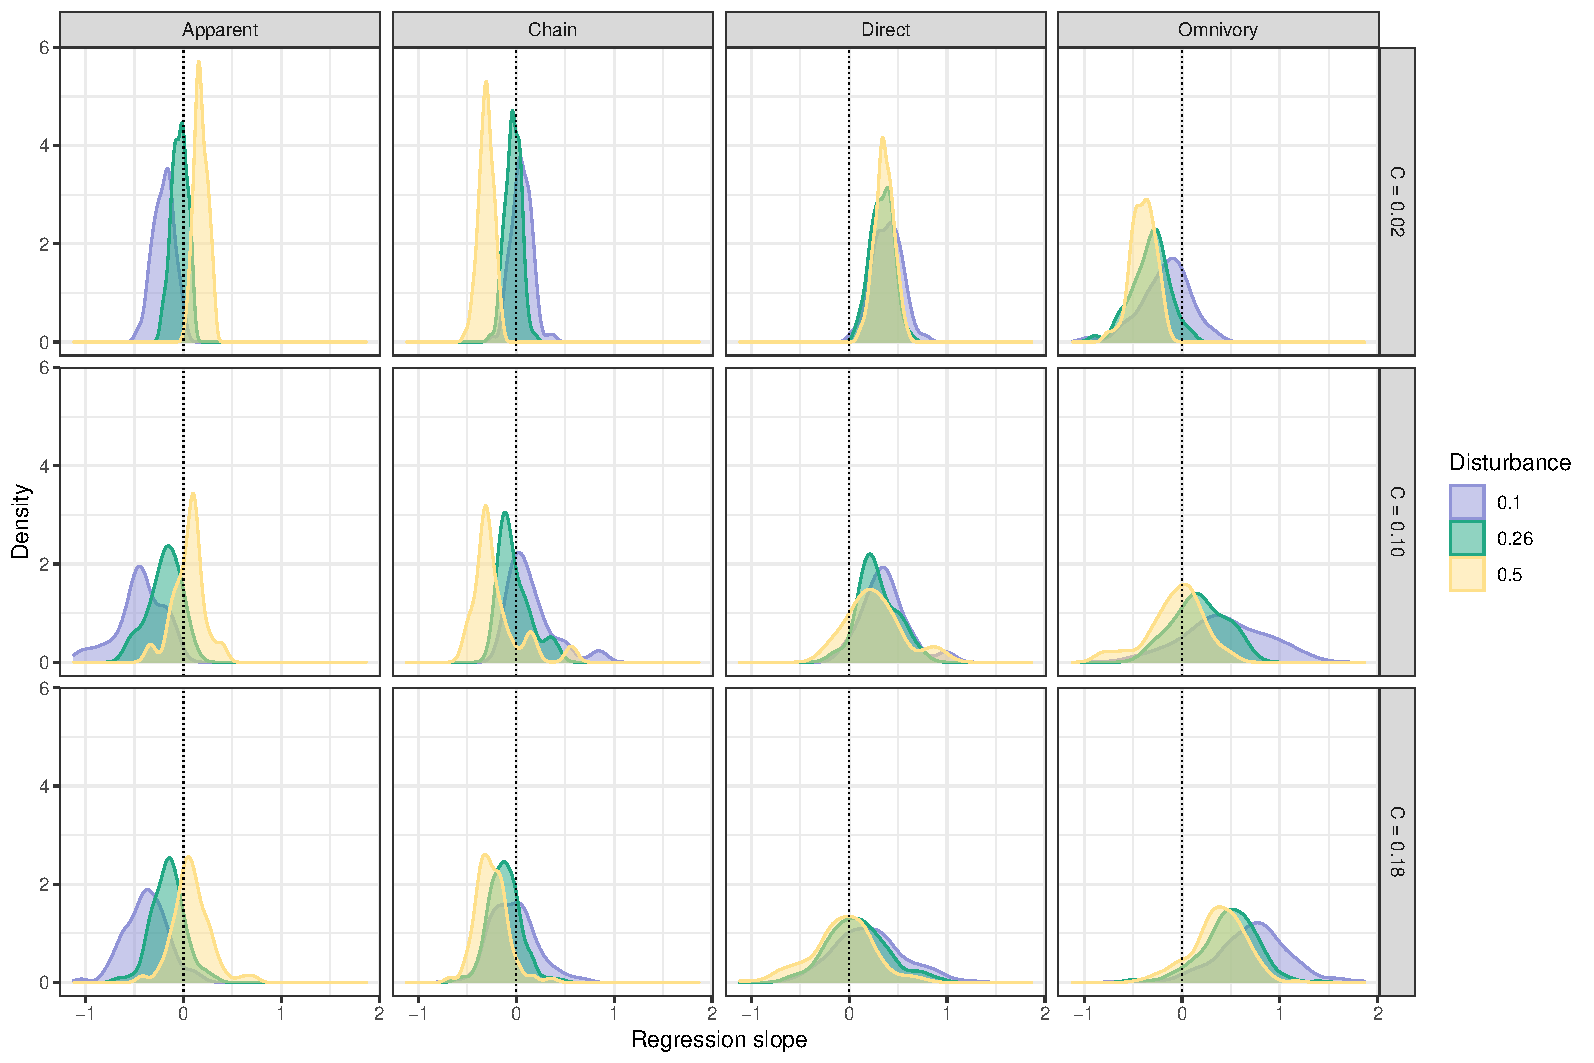
\includegraphics[width=\textwidth]{figures/Fig4.pdf}
        \caption{Here we show the density (y-axis) of slopes (x-axis) of persistence against proportion of different motifs for all simulated webs of all sizes - a visualization of how an increased proportion of each motif (different colored lines) affects persistence of consumer species. Columns show the result for various disturbances on the basal level, from $\pi_{disturbed} = 0.1$ (left) to $\pi_{disturbed} = 0.5$ (right). Rows show various levels of connectance. The dotted, vertical lines indicate zero on the x-axis. A negative slope value reflects a negative relationship between increased participation in a motif and persistence, while a positive slope value reflects a positive relationship - an increased proportion of a specific motif increases persistence. The fraction of replicates with a slope greater than zero are stated in numbers in each sub-plot, the color corresponding to each motif (legend). }
        \label{fig:density_prop}
    \end{figure}    


    \begin{figure}[ht!]
        \centering
        % \includegraphics[width=\textwidth]{figures/persistence_vs_SC_lm.eps}
        \caption{The probabilities of persistence for a particular consumer (\textbf{A, B}) and the average probability of persistence across all consumers (\textbf{C-E}) varied with other elements of network structure as well as with motif participation.
        \textbf{A} Persistence of consumers decreased with increasing STL at all levels of disturbance.
        \textbf{B} Persistence of consumers increased with increasing in-degree when the probability of extinction for basal resources was low but decreased with increasing in-degree when the probability of extinction was high.
        \textbf{C,D} Mean persistence of consumers in a network decreased strongly with increasing probability of disturbance to basal resources and decreased slightly, but significantly, with increasing connectance. There was no significant relationship between mean persistence and network size.
        \textbf{E} Mean persistence of consumers decreased with increasing proportions of omnivory in the network's motif profile and increased with increasing proportions of other motifs. Persistence also decreased significantly with increasing probability of basal species extinction but there was no significant interaction; we therefore show trends only for $\pi$=0.1.}
        \label{fig:lm_CS}
    \end{figure}

    \begin{figure}[hb!]
        \centering
        % \includegraphics[width=\textwidth]{figures/roles_vs_TL.eps}
        \caption{Motif participation correlated with in-degree and trophic level, and both of these simpler role measures were also correlated with persistence. \textbf{A)} The proportion of omnivory increased with increasing degree while all other proportions decreased. \textbf{B)} The proportions of omnivory and direct competition decreased with increasing STL while the proportions of apparent competition and three-species chains increased. \textbf{C-D)} The proportion of each motif in consumer's participation vectors varied with connectance, network size, and their interaction (except for apparent competition, where the interaction was not significant). To cover the largest range of slopes, we show relationships over connectance for the smallest networks (\textbf{C}) and over network size for the most-connected networks (\textbf{D}). See also Fig. SX. }
        \label{fig:motifs_vs_TL_and_deg}
    \end{figure}        



    % \begin{figure}[hb!]
    %     \centering
    %     \includegraphics[width=.9\textwidth]{figures/participation_vs_SC.eps}
    %     \caption{The proportion of each motif in consumer's participation vectors varied with connectance, network size, and their interaction (except for apparent competition). We show relationships for the smallest and largest values of network size (S) and connectance (C).}
    %     \label{fig:roles_vs_SC}
    % \end{figure}


    
    % \begin{figure}[hb!]
    %     \centering
    %     \includegraphics[width=\textwidth]{figures/persistence_motif_profiles.eps}
    %     \caption{The proportions of the four motifs in a network's motif profile are related to the mean persistence of species in the network. Specifically, persistence decreases as the proportion of omnivory in the network's motif profile increases while persistence increases with the proportion of the apparent competition motifs. Interactions between motif profiles and disturbance were not significant. Here we show the relationships of probabilities of extinction of basal resources of $\pi=0.1$ (top set of lines) and $\pi=0.5$ (bottom set of lines). Relationships are shown for the observed range of proportions for each motif.}      
    %     \label{fig:motif_profile_persistence}
    % \end{figure}    
    
    % \begin{figure}[hb!]
    %     \centering
    %     \includegraphics[width=\textwidth]{figures/motif_proportion_lms.eps}
    %     \caption{The proportion of the omnivory in a network's motif role increased significantly as connectance increased, while the proportions of the other three motifs did not vary significantly with network size, connectance, or their interaction.}
    %     \label{motif_proportion_lms}
    % \end{figure}




\clearpage

% \section*{Glossary}
% \begin{table}[h!]
% \label{glossary}
% \caption{Glossary of terms relating to motifs and Bayesian networks}
%     \footnotesize{
% \begin{tabular}{l|l}
%     Term & Definition \\
%     \hline
%     Motif & Set of $n$ interacting species. In this case, $n=3$ \\
%     Network motif profile & Vector describing the frequency of each motif in the network. \\
%     & Normalised by dividing counts of each motif by the total across all motifs.\\
%     Motif participation role & Vector describing the frequency with which a focal species appears in each motif.\\
%     & Normalised by dividing counts for each motif by the total across all motifs. \\
%     Bayesian network & A directed acyclic graph, used to predict species' likelihood of persistence. \\
%     Network persistence & The mean likelihood of consumers in a network not going extinct.\\
%     Species persistence & The individual likelihood of a species not going extinct.\\
%     In-degree & Number of prey species to a consumer species.\\
%     Trophic level (STL) & The shortest food chain between the focal species and any basal species.\\
%     Disturbance ($\pi_{disturbed}$) & Probability of extinction of a basal resource when extra disturbance is added. \\
%     Baseline extinction &  When no disturbance is applied, $\pi_{base}$=0.1.\\
% \end{tabular}}
% \end{table}

% Notes on what expressions and words to use
% "probability of extinction" or "level of disturbance" for the different disturbace scenarios?


\bibliographystyle{jae} 
\bibliography{anna_bib_new} % Abbreviate journal titles.

\end{spacing}

\end{document}

